% 第三章-问题建模
\section{Problem Description and Temporal Heterogeneous Graph Modeling}
\label{sec:problem}

% 3.1-问题描述
\subsection{Problem Description of Dynamic Manufacturing-Assembly Scheduling}
\label{subsec:problem_description}

% 问题定义与预备知识
% 描述研究问题的基本定义，包括系统中的实体对象、决策过程、
% 约束条件、动态事件以及优化目标。
% 明确列出建模过程中采用的假设，并对每个假设的合理性进行说明。

The considered scheduling problem is illustrated in Fig.~\ref{fig:problem_description}.

\begin{figure}[t]
  \centering
  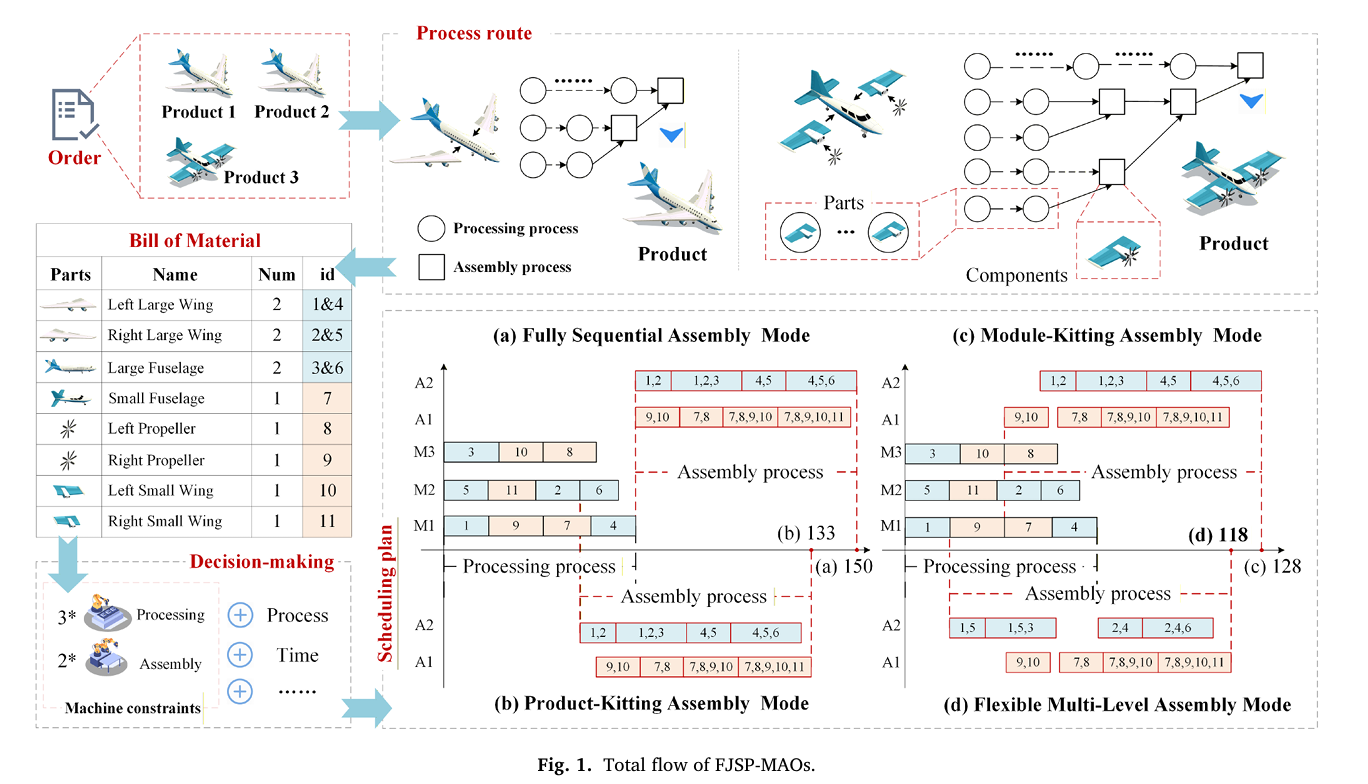
\includegraphics[width=0.9\textwidth]{figures/F1动态加工-装配调度场景图.png}
  \caption{Illustration of the considered scheduling problem.}
  \label{fig:problem_description}
\end{figure}


% 3.2-数学模型建模
\subsection{Mathematical Formulation of the Scheduling Problem}
\label{subsec:mathematical_model}

% 在建立数学模型前，首先定义集合、索引、参数以及决策变量。
% 将下面的通用数学模型替换为与本文问题完全对应的目标函数和约束条件。

\begin{equation}
  \min \; f(\boldsymbol{x})
  \label{eq:generic_objective}
\end{equation}

\begin{align}
  g_k(\boldsymbol{x}) &\le 0, && k \in \mathcal{K}, \\
  h_l(\boldsymbol{x}) &= 0, && l \in \mathcal{L}.
  \label{eq:generic_constraints}
\end{align}

% 3.3-图结构建模
\subsection{Temporal Heterogeneous Graph Representation}
\label{subsec:graph_representation}

Define the time-dependent heterogeneous graph as

\begin{equation}
  \graph=(\nodes,\edges,\phi,\psi),
  \label{eq:heterogeneous_graph}
\end{equation}

where $\phi$ and $\psi$ map nodes and edges to their types. Specify node types,
edge types, raw features, update timing, and how constraints are encoded.

% 添加一个图结构示意图，用于展示节点类型、边类型以及它们之间的语义关系。


% 定义马尔可夫决策过程（MDP）的基本形式，
% 并分别介绍状态（state）、动作（action）、
% 状态转移/决策时刻（transition/decision epoch）、
% 奖励函数（reward）以及终止条件（termination condition）。
